\startchapter{The DH Model}
\label{chapter:dh_model}

The dark matter (DM) search presented in this thesis is motivated by and interpreted with the ``Dark Higgs" (DH) model \cite{Duerr2017}. The DH model predicts a mechanism for DM production from proton-proton collisions at the LHC by means of portal interactions with the dark sector. The dark sector, which is predicted as part of various BSM models, represents a collection of quantum fields and associated particles which are assumed to interact gravitationally, but which do not couple via any of the other known forces - electromagnetic, strong and weak - of the SM. Non-gravitational couplings between the dark sector and the SM proceed instead via one or more so-called ``portal mediators". 

In the DH model, the DM is a particle which belongs to the dark sector, and is produced from high-energy \(q\bar{q}\) collisions at the LHC via a hypothetical spin 1 vector boson portal mediator referred to as the \Zprime. The model introduces an additional Higgs boson in the dark sector called the ``Dark Higgs" (DH), which acts as a portal mediator by decaying to SM particles via a small mixing with the SM Higgs boson. 

Figure \ref{fig:Feynman_DH} shows three Feynman diagrams \textcolor{red}{(Note to Bob/self: may need to briefly introduce Feynman diagrams in ch. 1)} which illustrate some of the dominant modes by which the DH model could produce a measurable signature of DM production at the LHC. In all cases, the DM pair is produced via the \Zprime mediator, along with the emission of a DH boson \(s\), which decays to a pair of SM particles. 

\begin{figure}[hp]
	\centering
	\begin{subfigure}[t]{0.49\textwidth}
	\centering
	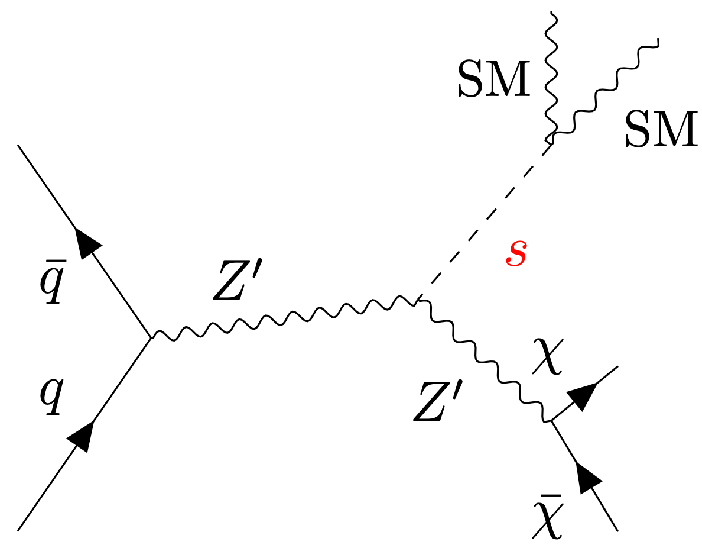
\includegraphics[width=0.95\textwidth]{Figures/2/Fey1.pdf}
	\label{fig:dh_schannel_1}
%		\begin{tikzpicture}
%			\begin{feynman}
%
%		 		\vertex (a1);
%		 		\vertex[below=7em of a1] (b1);
%		 		\vertex at ($(a1)!0.5!(b1) + (1cm, 0)$) (c1); %z'
%		 		\vertex at ($(a1)!0.4!(b1) + (3cm, 0)$) (c2); %z'
%
%		 		\vertex[right=4cm of a1] (a2); % s
%		 		\vertex[below=5em of a2] (b2); % z'
%
%		 		\vertex at ($(c2) + (1.5cm, 0) + (0,-0.5cm)$) (a3);
%		 		\vertex[below=3em of a3] (b3);
%
%		 		\vertex at ($(a2) + (0, 1cm)$) (a4) ;
%		 		\vertex at ($(a2) + (0, 0.8cm) + (0.8cm, 0)$) (b4) ;
%
%		 		\diagram* {
%		 		  {[edges=fermion]
%		 		    (b1) -- [edge label=\(q\)]( c1) -- [edge label=\(\bar{q}\)](a1),
%		 		    (b3) -- [edge label=\(\bar{\chi}\)] (b2) -- [edge label=\(\chi\)]  (a3),
%		 		  },
%		 		  (c1) -- [boson, edge label=\(Z'\)] (c2),
%		 		  (a2) -- [scalar,edge label=\(\color{red} s\)] (c2) -- [boson, edge label'=\(Z'\)] (b2),
%		 		  (a4) -- [boson, edge label'={\small SM}] (a2) -- [boson, edge label'=\small{SM}] (b4),
%
%		 		};
%		 	\end{feynman}
%		 \end{tikzpicture}
	\caption{s-channel (DH and DM emitted from the \Zprime)}
	\end{subfigure}
		\begin{subfigure}[t]{0.45\textwidth}
	\centering
	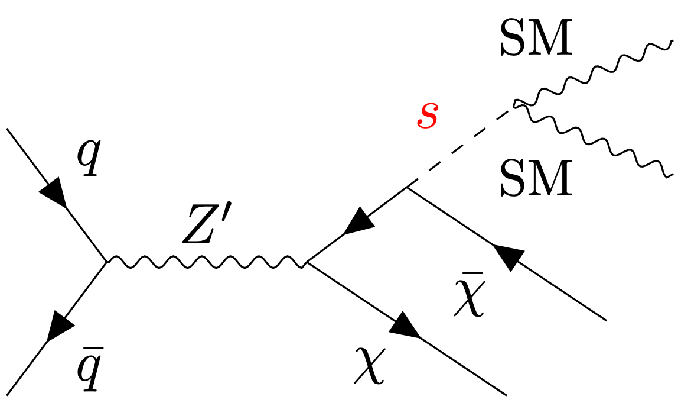
\includegraphics[width=0.95\textwidth]{Figures/2/Fey2.pdf}
%		\begin{tikzpicture}
%			\begin{feynman}
%
%		 		\vertex (b1);
%		 		\vertex at ($(b1) + (-0.75cm, 1cm)$) (a1); %q
%		 		\vertex at ($(b1) + (-0.75cm, -1cm)$) (a2); %qbar
%				\vertex at ($(b1) + (1.5cm, 0cm)$) (c1); %Z'
%				\vertex at ($(c1) + (1.5cm, -1cm)$) (d1); %chi
%				\vertex at ($(c1) + (0.75cm, 0.56cm)$) (d2); %chi
%				\vertex at ($(d2) + (1.5cm, -1cm)$) (d3); %chibar
%				\vertex at ($(d2) + (0.8cm, 0.6cm)$) (e1); %s
%				\vertex at ($(e1) + (1.2cm, 0.5cm)$) (f1); %W
%				\vertex at ($(e1) + (1.2cm, -0.5cm)$) (f2); %W
%				
%				\diagram* {
%				 (a1) -- [fermion, edge label=\(q\)](b1) -- [fermion, edge label=\(\bar{q}\)](a2),
%				 (b1) -- [boson, edge label=\(Z'\)] (c1),
%				 (d3) -- [fermion, edge label=\(\bar{\chi}\)](d2) -- [fermion](c1) -- [fermion, edge label'=\(\chi\)](d1),
%				 (d2) -- [scalar, edge label=\(\color{red} s\)] (e1),
%				 (f1) -- [boson, edge label'={\small SM}](e1) -- [boson, edge label'={\small SM}](f2),
%		 		};
%		 	\end{feynman}
%		 \end{tikzpicture}
	\label{fig:dh_schannel_2}
	\caption{s-channel (DM emitted from the \Zprime, DH emitted from the DM)}
	\end{subfigure}
	\begin{subfigure}[t]{.42\textwidth}
	\centering
	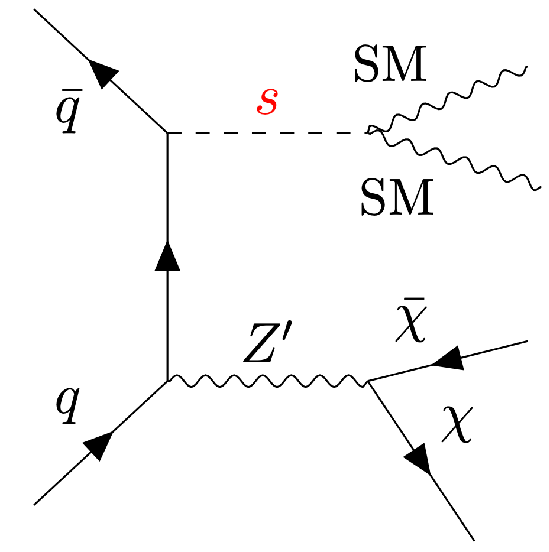
\includegraphics[width=0.95\textwidth]{Figures/2/Fey3.pdf}
%		 \begin{tikzpicture}
%		 	\begin{feynman}
%		 		\vertex (a1); %qbar
%		 		\vertex[below=9em of a1] (b1); %q
%				\vertex at ($(a1)!0.25!(b1) + (1cm, 0)$) (b5); %s
%		 		\vertex at ($(a1)!0.75!(b1) + (1cm, 0)$) (c1); %z'
%		 		\vertex at ($(c1) + (1.5cm, 0) + (0,0)$) (c2); %z'
%
%	         		\vertex[right=1.5cm of b5] (a2); % s
%		 		\vertex[below=2em of a2] (b2); % z'
%
%		 		\vertex at ($(c2) + (0.8cm, 0) + (0,-1.2cm)$) (a3);
%		 		\vertex at ($(c2) + (1.2cm, 0) + (0,0.3cm)$) (b3);
%
%		 		\vertex at ($(a2) + (1.2, 0.5cm)$) (a4) ;
%		 		\vertex at ($(a2) + (0, -0.4cm) + (1.3cm, 0)$) (b4) ;
%
%		 		\diagram* {
%		 		  {[edges=fermion, very thick]
%		 		    (b1) -- [edge label=\(q\)]( c1) -- (b5) -- [edge label=\(\bar{q}\)](a1),
%		 		    (b3) -- [edge label'=\(\bar{\chi}\)] (c2),
%		 		    (c2) -- [edge label=\(\chi\)]  (a3),
%		 		  },
%		 		  {[very thick]
%		 		  (c1) -- [boson, edge label=\(Z'\)] (c2),
%		 		  (b5) -- [scalar,edge label=\(\color{red} s\)] (a2),
%		 		  (a4) -- [boson, edge label'={\small SM}] (a2) -- [boson, edge label'={\small SM}] (b4),
%	         		  }
%		 		};
%		 	\end{feynman}
%		 \end{tikzpicture}
	\caption{t-channel (DH radiated off \(q\), DM emitted from the \Zprime)}
	\label{fig:dh_tchannel}
	\end{subfigure}
	\caption{The most contributing Feynman diagrams for DM production at the LHC by means of the DH model}
	\label{fig:Feynman_DH}
\end{figure}


\section{Theoretical Motivation for the Dark Higgs Model}

Given that the particles of the SM acquire mass via their interaction with the Higgs field \cite{HiggsTheory1,HiggsTheory2,HiggsTheory3}, the existence of a hypothetical ``DH" field - and its associated particle the DH boson - is motivated by the need to likewise generate the masses of particles in the dark sector. More generally, the existence of so-called portal mediators which enable interactions between dark sector and SM particles is motivated by theoretical arguments, discussed in Chapter \ref{chapter:introduction} \textcolor{red}{(Note to Bob/self: will point to specific section presenting the thermal freeze-out hypothesis once it's written)}, for the presence of thermal equilibrium between DM and SM particles in the early Universe \cite{DM_earlyUniverse}, which would be established by creation and annihilation processes between particles in the two sectors. The present-day relic abundance of DM, set at the time of thermal freeze-out, places constraints on the details of these creation and annihilation processes. The hypothesized DH boson would open up a new mechanism for portal interactions between DM and SM particles. As discussed in the following section, this new mechanism allows for a relaxation of constraints from the DM relic abundance compared with simpler models in which portal interactions are limited to those mediated by a vector boson mediator (the so-called \Zprime). 

\subsection{Constraints on Generic \Zprime Mediator Models} 
\label{sec:Zprime_model_constraints}

In addition to providing a mechanism by which particles acquire mass in the dark sector, the introduction of a new Higgs boson in the dark sector is motivated by strong theoretical and experimental constraints \cite{Zprime_portal_gen, Zprime_portal_monojet_dijet} on the more generic simplified model in which portal interactions between the dark sector and the DM are mediated exclusively by the \Zprime vector boson mediator. Removing the emission of the DH \(s\) from the contributing Feynman diagrams of the DH model in Figure \ref{fig:Feynman_DH} reduces all three to the generic ``s-channel" mechanism by which SM particles would pair-annihilate to form DM via the \Zprime mediator, shown in Figure \ref{fig:Feynman_Zprime_DM}. 

\begin{figure}[hp]
	\centering
\begin{subfigure}[t]{0.32\textwidth}
	\centering
	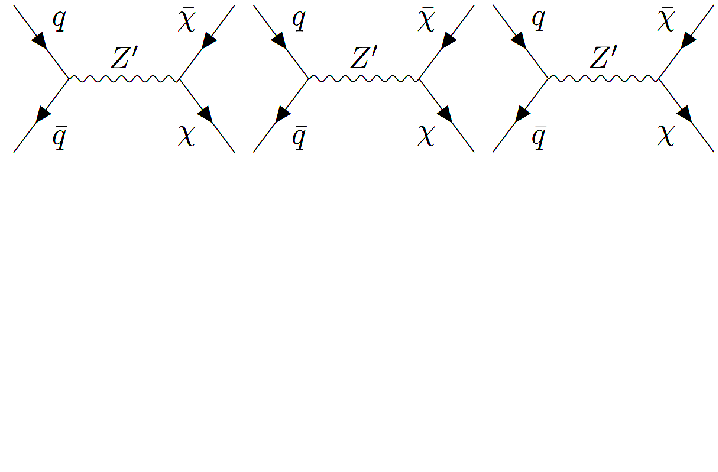
\includegraphics[width=0.8\textwidth]{Figures/2/FeyZprime.pdf}
%		\begin{tikzpicture}
%			\begin{feynman}
%
%		 		\vertex (b1);
%		 		\vertex at ($(b1) + (-0.75cm, 1cm)$) (a1); %q
%		 		\vertex at ($(b1) + (-0.75cm, -1cm)$) (a2); %qbar
%				\vertex at ($(b1) + (1.5cm, 0cm)$) (c1); %Z'
%				\vertex at ($(c1) + (0.75cm, -1cm)$) (d1); %chi
%				\vertex at ($(c1) + (0.75cm, 1cm)$) (d2); %chi
%				
%				\diagram* {
%				 (a1) -- [fermion, edge label=\(q\)](b1) -- [fermion, edge label=\(\bar{q}\)](a2),
%				 (b1) -- [boson, edge label=\(Z'\)] (c1),
%				 (d2) -- [fermion, edge label'=\(\bar{\chi}\)](c1) -- [fermion, edge label'=\(\chi\)](d1);
%		 		};
%		 	\end{feynman}
%		 \end{tikzpicture}
\caption{Generic DM production}
\label{fig:Feynman_Zprime_DM}
\end{subfigure}
\begin{subfigure}[t]{0.32\textwidth}
	\centering
	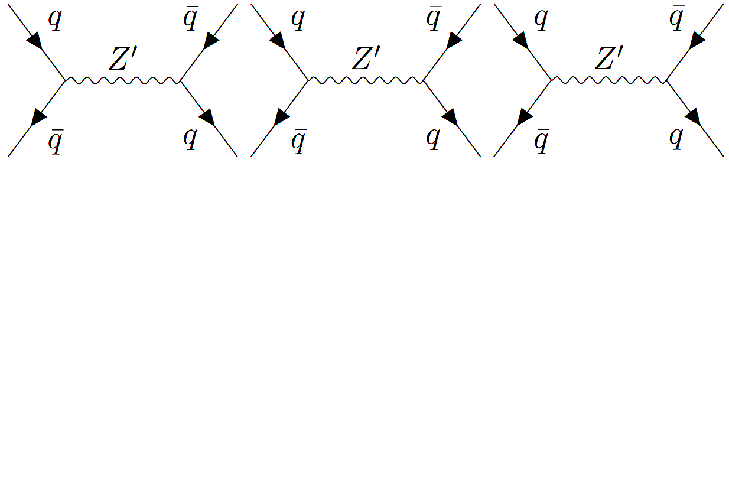
\includegraphics[width=0.8\textwidth]{Figures/2/FeyZprime_dijet.pdf}
%		\begin{tikzpicture}
%			\begin{feynman}
%
%		 		\vertex (b1);
%		 		\vertex at ($(b1) + (-0.75cm, 1cm)$) (a1); %q
%		 		\vertex at ($(b1) + (-0.75cm, -1cm)$) (a2); %qbar
%				\vertex at ($(b1) + (1.5cm, 0cm)$) (c1); %Z'
%				\vertex at ($(c1) + (0.75cm, -1cm)$) (d1); %chi
%				\vertex at ($(c1) + (0.75cm, 1cm)$) (d2); %chi
%				
%				\diagram* {
%				 (a1) -- [fermion, edge label=\(q\)](b1) -- [fermion, edge label=\(\bar{q}\)](a2),
%				 (b1) -- [boson, edge label=\(Z'\)] (c1),
%				 (d2) -- [fermion, edge label'=\(\bar{q}\)](c1) -- [fermion, edge label'=\(q\)](d1);
%		 		};
%		 	\end{feynman}
%		 \end{tikzpicture}
\caption{Dijet resonance}
\label{fig:Feynman_Zprime_dijet}
\end{subfigure}
\begin{subfigure}[t]{0.32\textwidth}
	\centering
	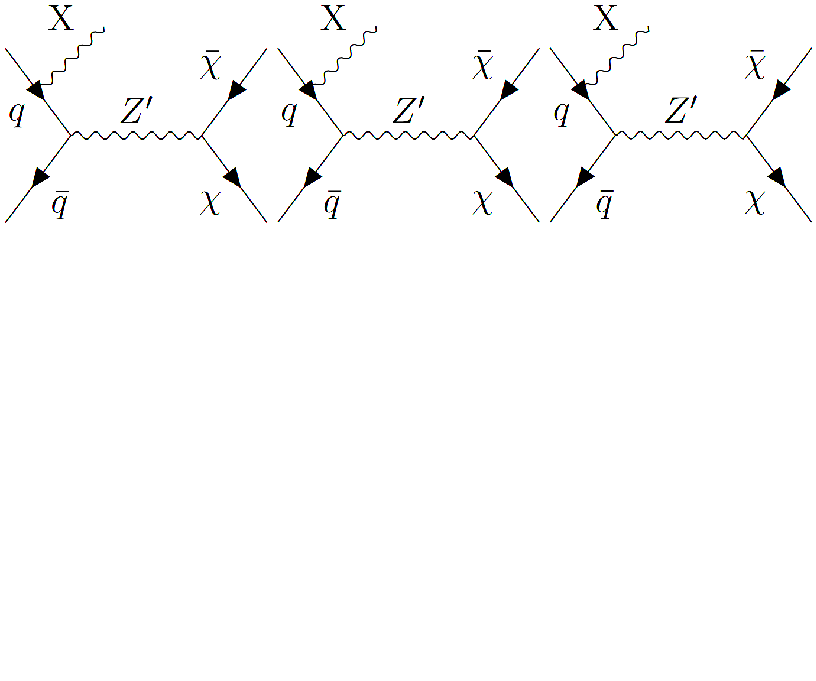
\includegraphics[width=0.8\textwidth]{Figures/2/FeyZprime_monoX.pdf}
%		\begin{tikzpicture}
%			\begin{feynman}
%
%		 		\vertex (b1);
%		 		\vertex at ($(b1) + (-0.75cm, 1cm)$) (a1); %q
%				\vertex at ($(b1) + (-0.375, 0.5cm)$) (s1); %SM
%				\vertex at ($(s1) + (0.75, 0.75cm)$) (s2); %SM
%		 		\vertex at ($(b1) + (-0.75cm, -1cm)$) (a2); %qbar
%				\vertex at ($(b1) + (1.5cm, 0cm)$) (c1); %Z'
%				\vertex at ($(c1) + (0.75cm, -1cm)$) (d1); %chi
%				\vertex at ($(c1) + (0.75cm, 1cm)$) (d2); %chi
%				
%				\diagram* {
%				 (a1) -- [fermion, edge label'=\(q\)](b1) -- [fermion, edge label=\(\bar{q}\)](a2),
%				 (s1) -- [boson, edge label=X,near end](s2),
%				 (b1) -- [boson, edge label=\(Z'\)] (c1),
%				 (d2) -- [fermion, edge label'=\(\bar{\chi}\)](c1) -- [fermion, edge label'=\(\chi\)](d1);
%		 		};
%		 	\end{feynman}
%		 \end{tikzpicture}
\caption{Mono-X signature}
\label{fig:Feynman_Zprime_monoX}
\end{subfigure}
	\caption{Signatures for DM production and detection via a Z' vector boson mediator at the LHC}
	\label{fig:Feynman_Zprime}
\end{figure}

The Z' mediator model is probed at the LHC using either dijet resonance searches \cite{Zprime_portal_gen} which look for a signature of a \Zprime being created and subsequently decaying back into a pair of quarks as shown in Figure \ref{fig:Feynman_Zprime_dijet}, or with so-called ``mono-X" searches \cite{Zprime_portal_monojet_dijet} in which a SM particle ``X" is emitted as initial state radiation from one of the colliding quarks, as shown in Figure \ref{fig:Feynman_Zprime_monoX}, to produce a signature of SM particles recoiling against missing transverse momentum due to the undetected DM pair \textcolor{red}{(Note to Bob/self: need to include brief intro to \met in ch. 1)}. 

Dijet resonance searches probe the model by searching for the presence of a resonant peak in the dijet invariant mass spectrum over the SM background of QCD-induced dijet events, where this above-background peak would be induced by the process in Figure \ref{fig:Feynman_Zprime_dijet}. Ref. \cite{Zprime_portal_dijet} presents a statistical combination of several dijet searches that were performed with the ATLAS and CMS detectors, as well as an interpretations of the observed absence of any such above-background resonance peaks in the context of the \Zprime mediator model. It is found that for typical choices of the coupling strengths \(g_q\) (\(g_\chi\)) between the \Zprime and quarks (DM), the model is excluded over a wide range of \Zprime masses (\(500~\GeV < \mZp < 3~\TeV\)) over nearly all DM masses up to 2 TeV, as shown in Figure \ref{fig:Zprime_constraints_dijet}. A statistical combination of monojet searches performed by ATLAS and CMS, in which the radiated particle X in Figure \ref{fig:Feynman_Zprime_monoX} is a quark or gluon, is presented in Ref. \cite{Zprime_portal_monojet_dijet}. As shown in Figure \ref{fig:Zprime_constraints_monojet}, the monojet searches likewise excludes a large region of DM and vector boson mediator masses for a range of choices of coupling constants \(g_q\) and \gchi.

\begin{figure}[hp]
	\centering
\begin{subfigure}[t]{0.45\textwidth}
	\centering
	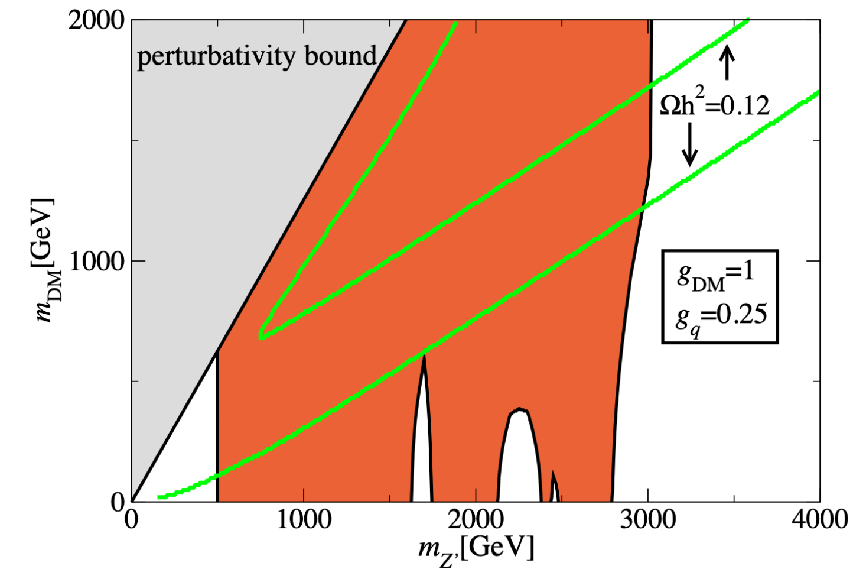
\includegraphics[width=0.9\textwidth]{Figures/2/Zprime_constrants_dijet.pdf}
\caption{Dijet resonance. Figure from $\copyright$ \cite{Zprime_portal_dijet}.}
\label{fig:Zprime_constraints_dijet}
\end{subfigure}
\begin{subfigure}[t]{0.54\textwidth}
	\centering
	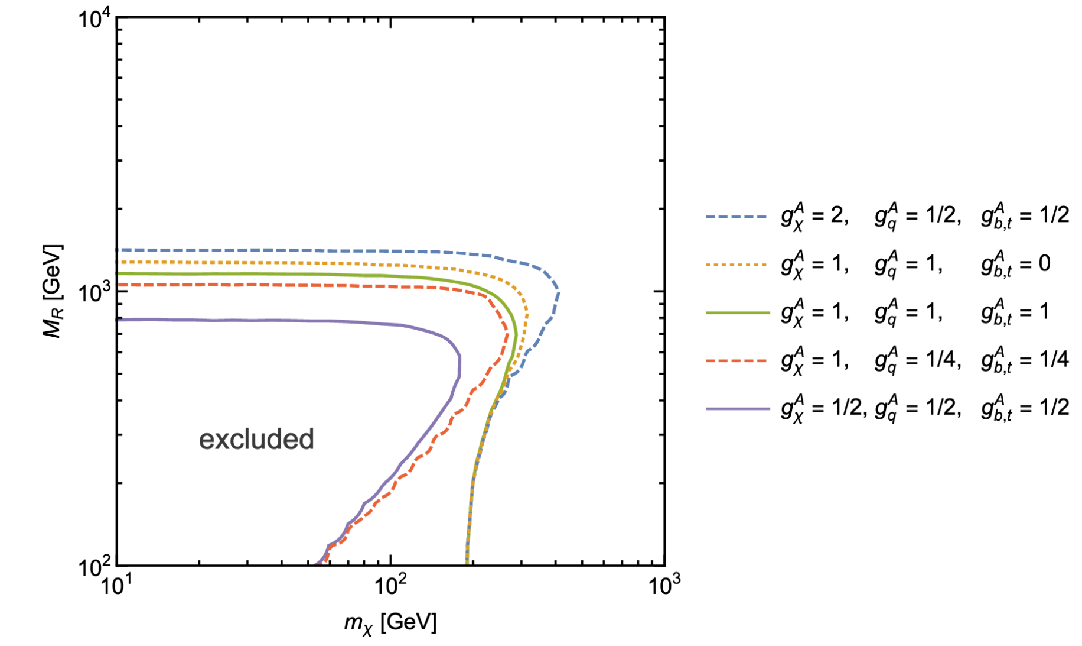
\includegraphics[width=0.99\textwidth]{Figures/2/Zprime_constrants_monojet.pdf}
\caption{Monojet. Figure from $\copyright$ \cite{Zprime_portal_monojet_dijet}.}
\label{fig:Zprime_constraints_monojet}
\end{subfigure}
	\caption{Constraints on the masses of the \Zprime vector boson mediator (labelled \mZp in \ref{fig:Zprime_constraints_dijet} and \(M_R\) in \ref{fig:Zprime_constraints_monojet}) and DM (labelled \(m_\text{DM}\) in \ref{fig:Zprime_constraints_dijet} and \(\mchi\) in \ref{fig:Zprime_constraints_monojet}) from combined ATLAS and CMS dijet searches \cite{Zprime_portal_monojet_dijet} (left) and monojet searches \cite{Zprime_portal_monojet_dijet} (right). The results are shown for typical coupling choices of the \Zprime to DM (\(g_\text{DM}\) in \ref{fig:Zprime_constraints_dijet} and \(g^A_\chi\) in \ref{fig:Zprime_constraints_monojet}), and of the \Zprime to quarks (\(g_q\) in \ref{fig:Zprime_constraints_dijet} and \(g^A_q\) or  \(g^A_{b,t}\) in \ref{fig:Zprime_constraints_monojet}, where \(g^A_{b,t}\) specifies the coupling to heavy quarks, which may be 0 for models which prohibit heavy quark couplings). Green lines in \ref{fig:Zprime_constraints_dijet} contain the region of \(\mZp, ~\mchi\) which reproduces the observed relic density of DM in the Universe. In the grey region perturbative unitarity \cite{Zprime_portal_monojet_dijet} is violated.}
	\label{fig:Feynman_Zprime}
\end{figure}

\subsection{Implications of a Dark Higgs Portal}

The implications of introducing a new portal interaction mediated by a spin 0 boson (the DH) - which couples to the SM via a mixing with the SM Higgs boson - to the generic \Zprime mediator portal model are studied in detail by Duerr et al. in Ref. \cite{Duerr_2016}. In this study, it is found that within various regimes of the coupling strengths and masses of the hypothetical particles - the \Zprime, DH and DM - in this two-mediator model, referred to as the DH model, it is possible to relax or evade some of the constraints described above on the generic \Zprime mediator model from the combination of experimental results and the observed relic DM density in the Universe. As a result, in addition to providing a mechanism by which particles acquire mass in the dark sector, the DH also introduces new parameter space to the model that is not yet excluded by existing constraints. In particular, for \(\ms < 2\mchi\) and provided there are no other lighter particles in the dark sector, the only available decay route for the \(s\) is to SM particles via mixing with the SM Higgs, regardless of the mixing strength. In this case, the DM relic abundance is predominately set by the process \(\chi\chi\rightarrow ss\) followed by decays of \(s\) into SM particles, which allows for a significant relaxation of relic density constraints. 

For various choices of \mchi, Duerr et al. \cite{Duerr_2016} consider a range of \ms and \mZp, and perform global scans over all other free parameters in the DH model (see Section \ref{sec:DH_model_description} below), as shown in Figure \ref{fig:Duerr_general_constraints}, to identify regions in which the model has not yet been excluded by existing constraints. Particularly for \(\mchi\geq200 ~\GeV\), it is found that the model evades all existing constraints for a large region of \ms and \mZp (up to \(\sim1000~\GeV\) in \ms and up to \(\sim2500~\GeV\) in \mZp).

\begin{figure}[hp]
	\centering
	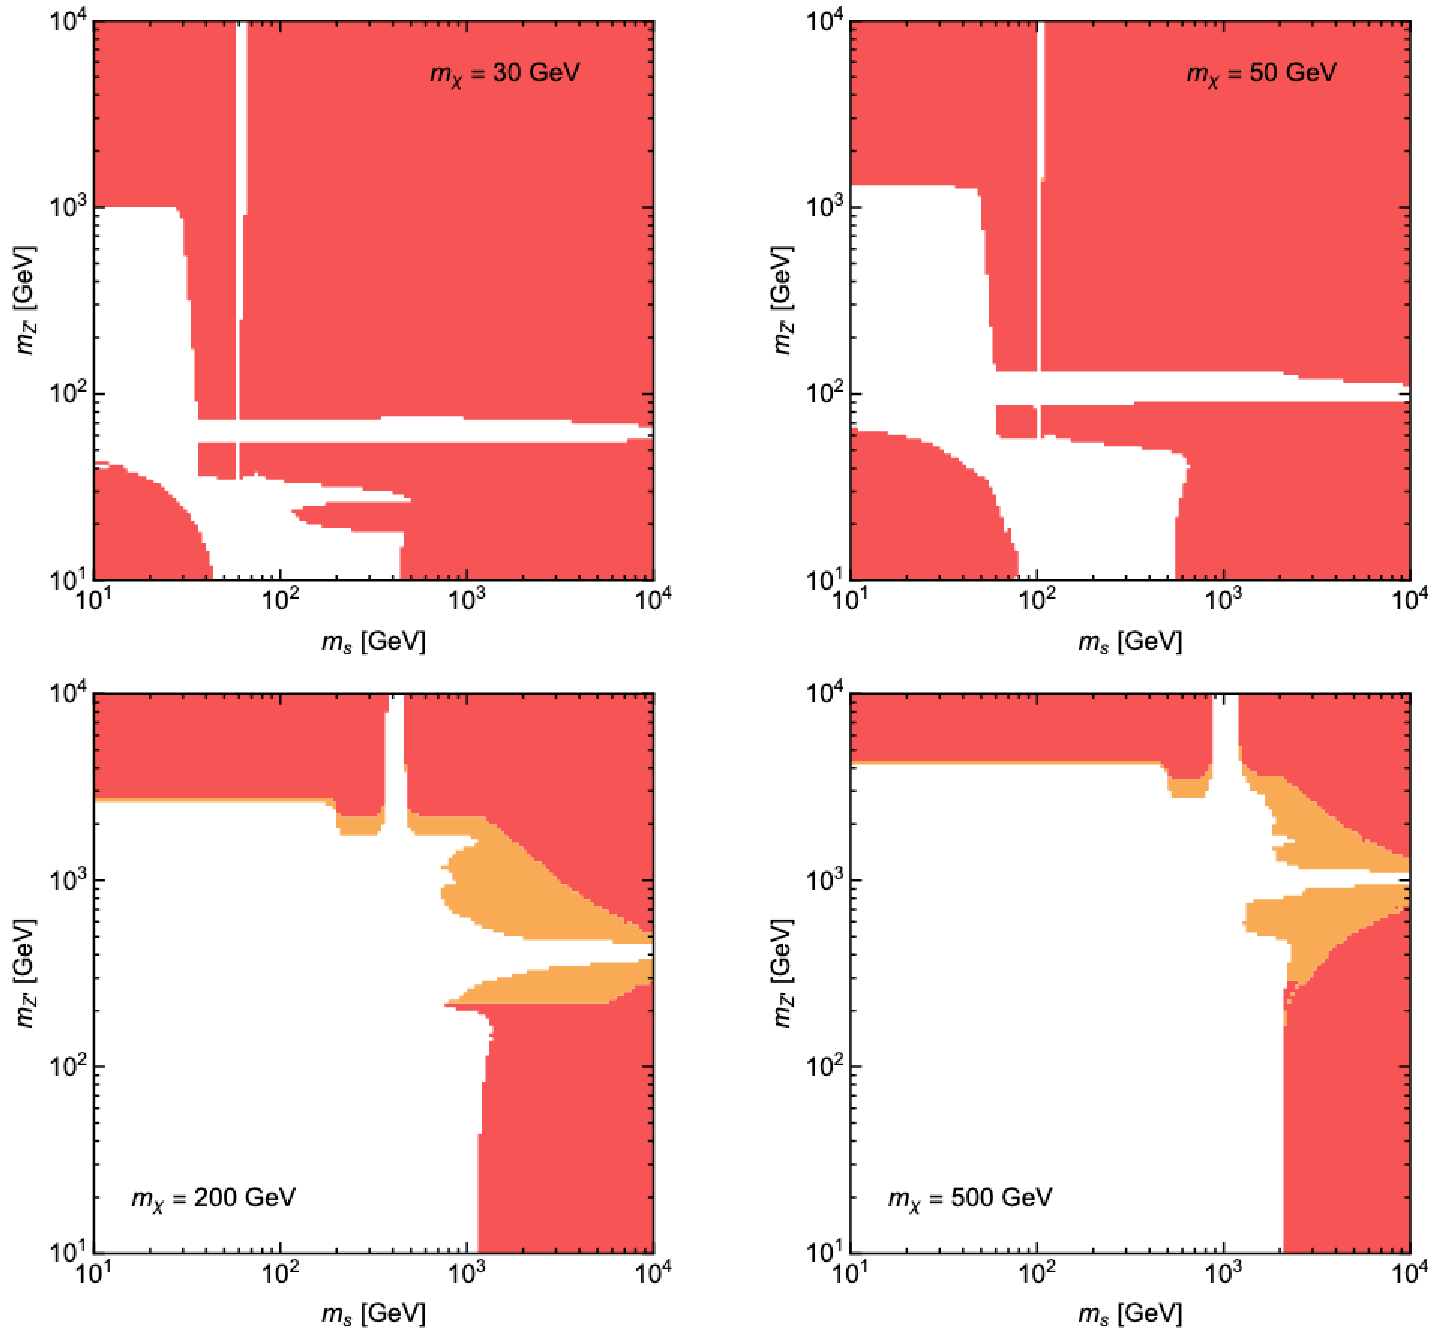
\includegraphics[width=0.8\textwidth]{Figures/2/Duerr_general_constraints.pdf}
	\caption{Global scans of the DH model, with \Zprime and DH as portal mediators, performed by Duerr et al in Ref. \cite{Duerr_2016}. The red shaded region is excluded for all possible
combinations of couplings, while in the white region all constraints can be evaded. In the orange shaded region it is not possible to exclude large values of \(g_q\) , corresponding to \(\Gamma_\Zprime / \mZp > 0.3\). Figure from $\copyright$ \cite{Duerr_2016}.}
	\label{fig:Duerr_general_constraints}
\end{figure}

\section{Model Description}
\label{sec:DH_model_description}

The DH model presented in Refs. \cite{Duerr_2016} and \cite{Duerr2017} belongs to a wider class of simplified dark sector models which hypothesize that DM interacts with particles of the SM via the exchange of one or more new mediators, which act as so-called ``portals" between the SM and the dark sector. Candidate portals are broadly categorized according to the portal mediator into vector- \cite{vector_mediator_2012,vector_mediator_2020}, neutrino- \cite{neutrino_mediator_2019}, Higgs- \cite{higgs_mediator_2020} and axion-mediated \cite{axion_mediator_2009} portals. In the DH model, DM is assumed to be a Majorana fermion, which means that - like the photon, for example - it is its own antiparticle, and interacts with the SM via both vector-mediated and Higgs-mediated portals. 

A new gauge group called the U(1)', with an associated vector gauge boson referred to as the \Zprime, is introduced as an extension of the SM gauge group presented in Chapter \ref{chapter:introduction}. Both the DM and and the \Zprime are assumed to acquire their mass from a new Higgs field with vaccum expectation value \(w\), which gives rise to a new physical Higgs boson, the DH boson \(s\). The DM acquires an axial coupling to the \Zprime, such that all three dark sector particles interact with one another. 

The interactions of the U(1)' gauge group within the dark sector are expressed by the interaction Lagrangian (of which more details can be found in Appendix A of Ref. \cite{Duerr_2016}):

\begin{equation}
\label{eq:DH_Lagrangian}
    \mathcal{L}_{U(1)'} = - \frac{1}{2} \gchi {\Zprime}^{\mu} \bar{\chi} \gamma^{5} \gamma_{\mu} \chi - \gchi \frac{\mchi}{\mZp} s \bar{\chi} \chi + 2 \gchi {\Zprime}^{\mu} {\Zprime}_{\mu} (\gchi s^2 + \mZp s)
\end{equation}

\noindent Considering each term in \(\mathcal{L}_{\chi}\) individually: 

\begin{equation}
\mathcal{L}_{\chi, \Zprime} = - \frac{1}{2} \gchi {\Zprime}^{\mu} \overline{\chi} \gamma^{5} \gamma_{\mu} \chi
\end{equation}

\noindent describes the axial coupling between the DM \(\chi\) and the \Zprime, with coupling strength \(g_\chi\). 

\begin{equation}
\label{eq:Lagrangian_chi_s}
\mathcal{L}_{\chi, \text{DH}} =- \gchi \frac{\mchi}{\mZp} s \bar{\chi} \chi = - \frac{y_\chi}{2\sqrt{2}} s \bar{\chi} \chi
\end{equation}

\noindent describes the coupling between the DM \(\chi\) and the DH field, where the associated coupling strength \(y_\chi\) on the right-hand side of Eq. \ref{eq:Lagrangian_chi_s} has the following dependence on the masses and coupling strength of the DM and the \Zprime: \(y_\chi = 2\sqrt{2}g_\chi\frac{\mchi}{\mZp}\).

\begin{equation}
\mathcal{L}_{\Zprime, \text{DH}} = 2 \gchi {\Zprime}^{\mu} {\Zprime}_{\mu} (\gchi s^2 + \mZp s)
\end{equation}

\noindent describes the interaction between the \Zprime and the DH field.

Motivated by models of gauged baryon number \cite{baryon_number,Duerr_2016,Duerr2017}, the SM quarks are charged under the U(1)' gauge group, and as a result have vector couplings with the \Zprime, which are described by the following interaction Lagrangian:

\begin{equation}
\label{eq:quark_Zprime_coupling}
\mathcal{L}_{q, \Zprime} = -g_q{\Zprime}^\mu\bar{q}\gamma_\mu q
\end{equation}

\noindent The quark-\Zprime coupling provides a mechanism for vector-mediated portal interactions between the SM and the dark sector. Axial vector couplings of the \Zprime to quarks would also be expected to produce a signature at the LHC, but are neglected in the model for simplicity \cite{Duerr2017}. 

 The most general Lagrangian describing the scalar Higgs \(h\) and DH \(s\) is given by \cite{DH_SMHiggs_mixing_2016}:
 
 \begin{equation}
 \label{eq:scalar_lagrangian}
 \mathcal{L}_\mathcal{\text{scalar}} = -\lambda_h \Big(H^\dagger H - \frac{v^2}{2}\Big) - \lambda_s \Big(S^\dagger S - \frac{w^2}{2}\Big) - \lambda_{hs} \Big(H^\dagger H - \frac{v^2}{2}\Big) \Big(S^\dagger S - \frac{w^2}{2}\Big)
 \end{equation}
 
\noindent where \(H=\frac{1}{\sqrt{2}}(0, v+h)\) represents the SM Higgs field with vacuum expectation value \(h\), and \(S=\frac{1}{\sqrt{2}}(s+w)\) represents the DH field. The third term with coupling \(\lambda_{hs}\) mixes the visible and dark sectors, such that the physical mass eigenstates \(h'\) and \(s'\) will be a superposition of the scalars \(h\) and \(s\):

\begin{equation}
\label{eq:higgs_mass_eigenstates}
\begin{pmatrix}
h' \\ s'
\end{pmatrix} = 
\begin{pmatrix}
\cos\theta & \sin\theta \\
\sin\theta & \cos\theta 
\end{pmatrix}
\begin{pmatrix}
h \\ s
\end{pmatrix}
\end{equation}

\noindent where the ``mixing angle" \(\theta\) is related to SM and DH field couplings \(\lambda_h\) and \(\lambda_s\) and the vacuum expectation values \(v\) and \(w\) by:

\begin{equation}
\label{eq:higgs_mixing_angle}
\tan2\theta = \frac{\lambda_{hs}vw}{\lambda_hv^2  \lambda_sw^2}
\end{equation}

Therefore, if the mixing between the SM and DH fields is nonzero (\(\sin\theta > 0\)), the physical Higgs eigenstate in the SM Lagrangian becomes \(h\cos\theta + s\sin\theta\). This opens up the possibility for interactions between the physical DH and SM particles, with coupling strengths scaled by \(\sin\theta\). For example, the Lagrangians describing the decay of the DH to SM fermions \(f\) and vector bosons \(V\) are described by \cite{Duerr_2016, PDG_2018}:  

\begin{equation}
\mathcal{L}_{hf\bar{f}} = -g_{hf\bar{f}}\bar{f}f h\sin\theta 
\end{equation}

\noindent and

\begin{equation}
\mathcal{L}_{hVV} = -\delta_V g_{hVV}V_\mu V^\mu h\sin\theta 
\end{equation}

\noindent where (from SM physics):

\begin{equation}
g_{hf\bar{f}} = \frac{_f}{v}, ~ g_{hVV} = \frac{2m_V^2}{v}, ~ \delta_W = 1, ~ \delta_Z = \frac{1}{2}
\end{equation}

\subsection{Free Parameters in the Model}
\label{sec:dh_model_free_parameters}

The free parameters in the DH model are as follows:

%\medskip\noindent\textbf{Sum of Weights Normalization}
\begin{itemize}
\item \(\mathbf{m_\chi}\): The mass of the DM particle \(\chi\).
\item \(\mathbf{m_{\Zprime}}\): The mass of the hypothetical \Zprime boson in the dark sector which mediates interactions between SM quarks \(q\) and the DM \(\chi\).
\item \(\mathbf{m_s}\): The mass of the hypothetical DH boson, whose associated Higgs field provides a mechanism for particles in the dark sector to acquire mass, and which can decay to SM particles via a small mixing with the SM Higgs boson.
\item \(\mathbf{g_q}\): Strength of the vector coupling between SM quarks and the \Zprime boson.
\item \(\mathbf{g_\chi}\): The coupling strength between DM and the \Zprime boson.
\item \(\mathbf{\theta}\): The mixing angle between the DH and the SM Higgs boson. The coupling strength associated with the decay of the DH to SM particles scales with \(\sin\theta\).
\end{itemize}

Some of these parameters are already constrained by other results. Mixing between the DH and the SM Higgs in the model would introduce unobservable decay modes of the SM Higgs to dark sector particles, which would modify the observed yield of Higgs events observed at the LHC from the SM expectation. Given the observed agreement between the observed yield and the SM expectation \cite{ATLAS-CONF-2020-027,CMS-PAS-HIG-19-005}, an upper limit of \(|\sin\theta| < 0.25\) can be placed \cite{Collider_searches_2021} (assuming no other appreciable unobserved decay channels exist).

Dijet resonance searches, discussed in Section \ref{sec:Zprime_model_constraints}, also place upper bounds on the coupling strength \(g_q\) of the \Zprime to SM quarks by searching for a resonant peak in the dijet spectrum associated with the scenario shown in Figure \ref{fig:Feynman_Zprime_dijet} in which a \Zprime is produced by high-energy \(q\bar{q}\) collisions at the LHC, and decays immediately back to a pair of quarks. Based on the agreement with SM predictions observed in the most recent dijet resonance searches performed by the ATLAS and CMS experiments \cite{dijet_1,dijet_2,dijet_3,dijet_4} limits on \(g_q\) ranging from 0.04 to 0.4, depending on \mZp, have been established. Figure \ref{fig:Dijet_gq_limits} shows upper bounds from two recent dijet searches, one of which (Figure \ref{fig:dijet_gq_limits_ATLAS}) uses ``trigger-level jets" \cite{dijet_2} to boost sensitivity in the low-\mZp range. 

\begin{figure}[hp]
	\centering
\begin{subfigure}[t]{0.57\textwidth}
	\centering
	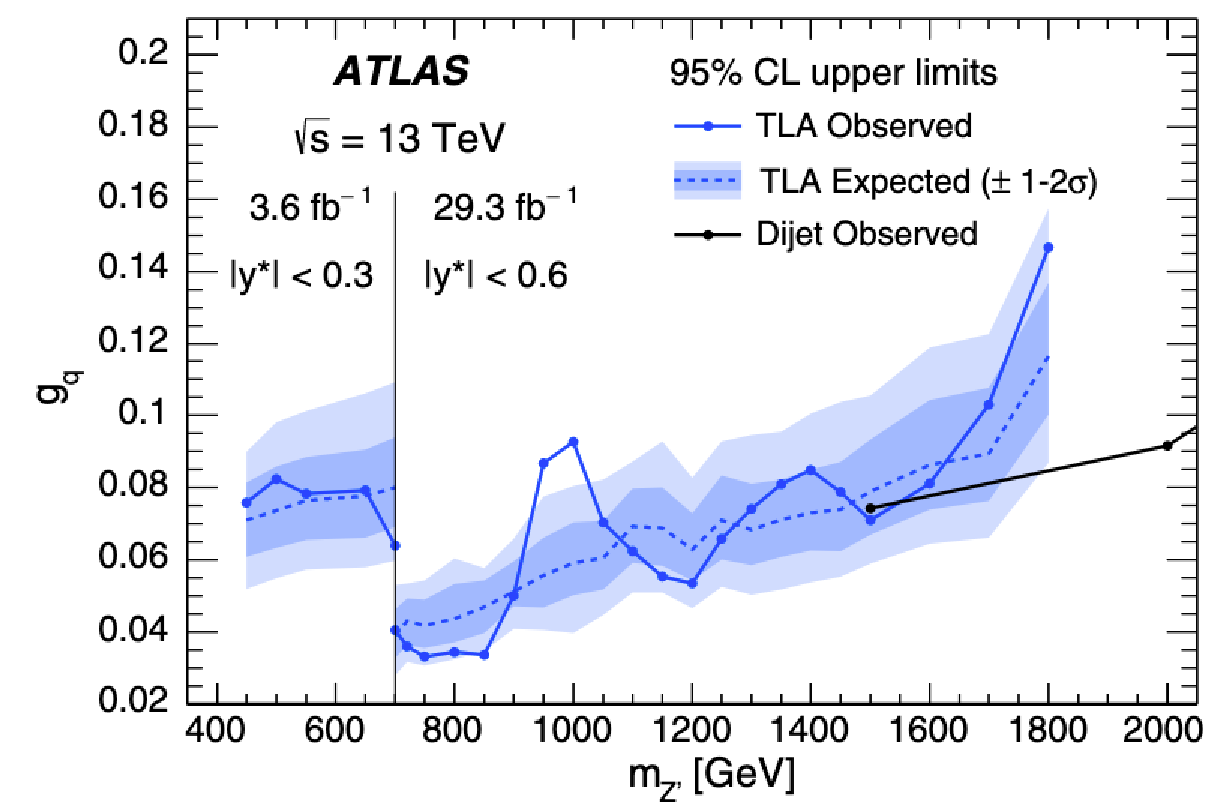
\includegraphics[width=0.9\textwidth]{Figures/2/Dijet_limits_ATLAS.pdf}
\caption{Limits from ATLAS low-mass dijet resonance search. Figure from $\copyright$ \cite{dijet_2}.}
\label{fig:dijet_gq_limits_ATLAS}
\end{subfigure}
\begin{subfigure}[t]{0.41\textwidth}
	\centering
	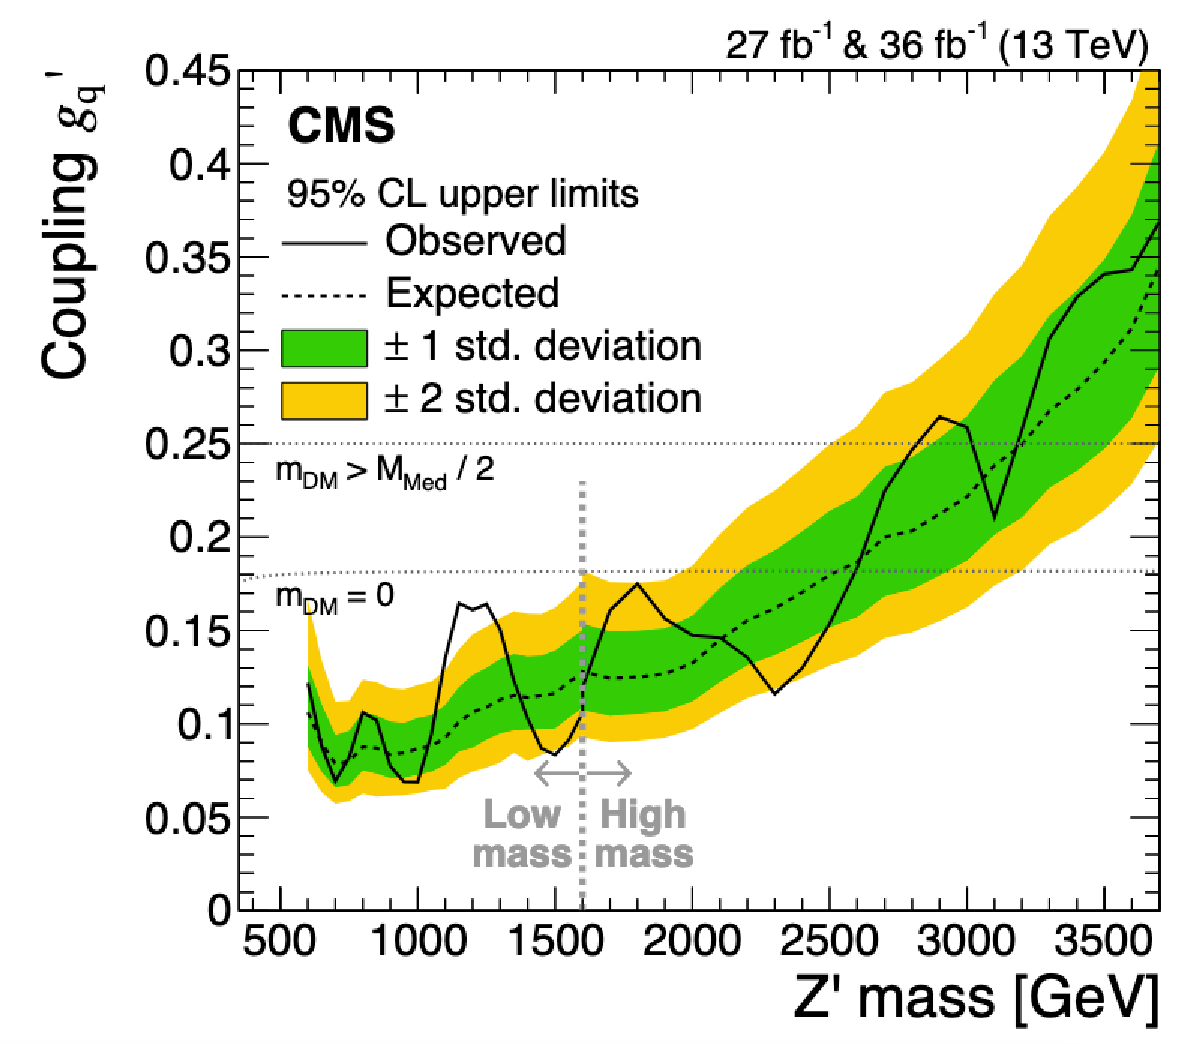
\includegraphics[width=0.99\textwidth]{Figures/2/Dijet_limits_CMS.pdf}
\caption{Limits from recent CMS search. Figure from $\copyright$ \cite{dijet_3}.}
\label{fig:dijet_gq_limits_CMS}
\end{subfigure}
	\caption{Upper bounds on the \(g_q\) coupling between the \Zprime and quarks, as reported by recent dijet resonance searches performed by ATLAS (left) and CMS (right).}
	\label{fig:Dijet_gq_limits}
\end{figure}

\section{Search for the Dark Higgs Model at the LHC}
\label{sec:dh_search_lhc}

For certain choices of the model parameters discussed in Section \ref{sec:dh_model_free_parameters}, the DH model predicts a unique and measurable signature by which it could be detected at the LHC. The signature, of which some of the most contributing Feynman diagrams are shown in Figure \ref{fig:Feynman_DH}, would occur when high-energy \(q\bar{q}\) in the colliding protons pair-annihilate to produce a \Zprime, which subsequently decays to DM. A measurable signature comes from the emission of a DH \(s\) either from a \(q\) or the \Zprime, which subsequently decays to a pair of SM particles. This produces a final state with the SM products from the \(s\) decay recoiling against \met in the detector due to the undetected DM pair \textcolor{red}{(Note to Bob: will include brief intro to \met in Ch. 1)}. In particular, assuming that the \Zprime is relatively low in mass compared with the centre of mass energy of the \(q\bar{q}\) collision, the \Zprime may be imparted with a large momentum (a.k.a. boost). As a result, the diagrams shown in Figures \ref{fig:dh_schannel_1} and \ref{fig:dh_schannel_2} in which the \(s\) is emitted from the \Zprime can produce highly boosted, collimated SM decay products from the boosted system, which make the signature distinct from typical mono-X final states in which the SM products (`X') recoiling against the DM are assumed to be produced exclusively as initial state radiation, as in Figure \ref{fig:dh_tchannel}.

\subsection{Dark Higgs Decay Channels}

As discussed in Section \ref{sec:DH_model_description}, since the DH decays to SM particles via mixing with the SM Higgs boson, its decay mechanisms - including its branching fractions for its various decay channels to different SM particles - will be analogous to that of the SM Higgs. As a result, the signature of boosted SM decay products recoiling against \met may be used to probe various ranges of \ms in the model depending on the particular choice of SM products (a.k.a. ``decay channel", or simply ``channel") from the \(s\) decay that the search targets. Figure \ref{fig:higgs_branching_fractions} shows the branching fraction that the SM Higgs - and consequently the DH \(s\) - would be expected to have to SM particles if its mass were allowed to float in the SM. For low \ms, the decay to \(b\bar{b}\) is dominant. At \(\ms\approx160~\GeV\), the decay to \(WW\) becomes kinematically accessible\footnote{A particular decay mode \(X\rightarrow YY\) generally becomes kinematically accessible for \(m_X > 2 m_Y\), because in this regime the on-shell parent particle \(X\) has a sufficient rest mass energy to decay to the daughter products \(YY\) while satisfying energy conservation.}, and is the dominant \(s\) decay channel for \(\ms\gtrsim160~\GeV\). The decay to \(ZZ\) also becomes kinematically accessible at \(\sim180~\GeV\), though its branching fraction remains sub-dominant compared with the \(WW\) decay. The decay to SM Higgses \(s\rightarrow HH\) opens up \(\sim250~\GeV\), above which this decay mode becomes appreciable, though still smaller than the \(WW\) mode. This suggests that searches in all four of these \(s\) decay channels could complement one another to collectively probe the full available \ms range, as summarized in Table \ref{tab:signal_grid_comparison}.

\begin{table}[hp]
\centering
\caption{Summary of DH decay channels to SM particles that could be targeted to probe various \ms ranges in DH model}
\label{tab:signal_grid_comparison}
\begin{tabular}{l l }
\toprule
\textbf{\(\mathbf{\ms}\) Range} & \textbf{Sensitive DH Decay Channels} \\
\midrule
\midrule
\(\ms < 160~\GeV\) & \(s\rightarrow bb\) \\
\midrule
\(160~\GeV < \ms < 180~\GeV\) & \(s\rightarrow WW\) \\
\midrule
\(180~\GeV < \ms < 250~\GeV\) & \(s\rightarrow WW\), \(s\rightarrow ZZ\) \\
\midrule
\(\ms >  250~\GeV\) & \(s\rightarrow WW\), \(s\rightarrow ZZ\), \(s\rightarrow HH\) \\
\bottomrule
\end{tabular}
\end{table}

\begin{figure}[hp]
	\centering
	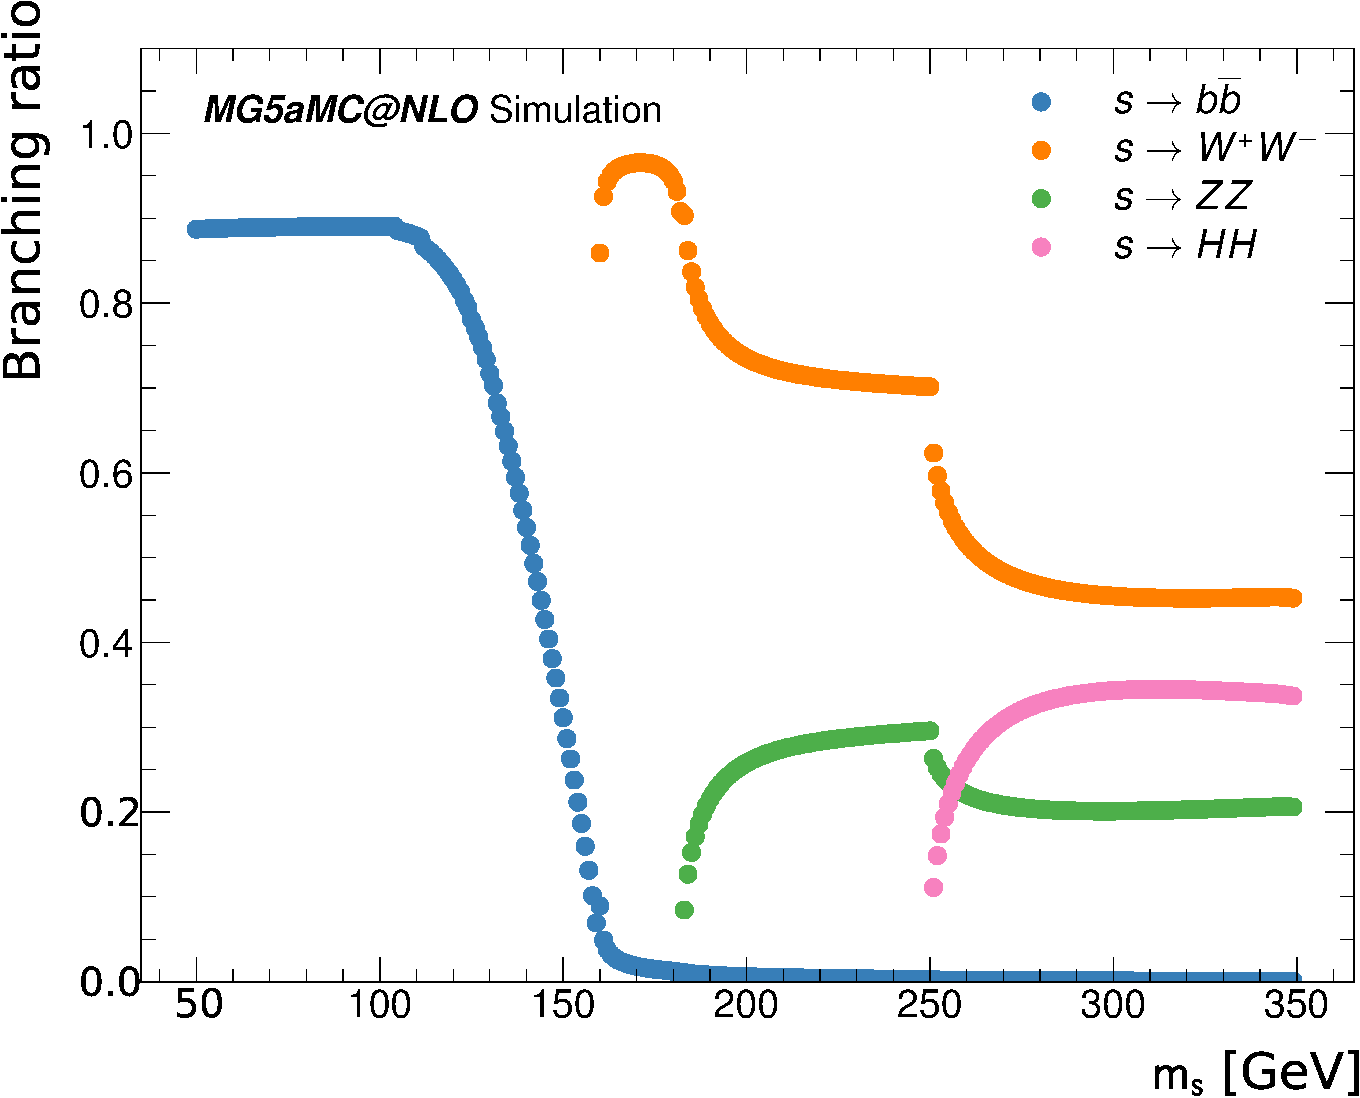
\includegraphics[width=0.6\textwidth]{figures/2/branchingratio.pdf}
	\caption{Branching fraction of the DH boson to SM particles in dependence of \ms. The branching fractions of the \(s\rightarrow WW\) and \(s \rightarrow ZZ\) decay modes experience a drop-off at  \(\ms=2 m_H (= 250~\GeV)\), above which the decay to \(s \rightarrow HH\) to SM Higgs becomes kinematically accessible.}
	\label{fig:higgs_branching_fractions}
\end{figure}

\subsection{Completed and Ongoing Searches for the Dark Higgs Model}

The search presented in this thesis is one of several existing searches for the DH model at the LHC, which target different decay modes of the DH \(s\) emitted in the model's LHC signatures shown in Figure \ref{fig:Feynman_DH}. 

\subsubsection{Model Parameters Probed by LHC Searches}

Given the number of parameters in the DH model, computational resource limitations make it impractical to scan over all parameters when performing dedicated searches for the model at the LHC. Therefore, in the search presented in this thesis - and in all other searches for the model performed to date at the LHC - the coupling constants and mixing angle \(\theta\) are fixed as follows:

\begin{itemize}
\item \(g_q=0.25\)
\item \(g_\chi=1\)
\item \(\sim\theta=0.01\)
\end{itemize}

The choice of \(|\sin\theta|=0.01\) is well within the range \(|\sin\theta|<0.25\) enforced by measurements of the SM Higgs - see above discussion in Section \ref{sec:dh_model_free_parameters}. The values of the coupling constants \gchi and \(g_q\) are chosen to be consistent - and thereby facilitates comparison with - other searches performed at the LHC for dark sector models involving a \Zprime mediator \cite{LHC_benchmarks_2020}. It is worth noting that the choice of \(\gchi=0.25\) is in fact ruled out in the approximate range \(500~\GeV < \mZp < 3000~\GeV\) by the recent dijet searches discussed above in Section \ref{sec:dh_model_free_parameters}. However, this choice is maintained in this search because it is considered important to maintain consistency with other searches performed with the same benchmark choices, and in particular it allows for the search results to be easily compared with other searches for the DH model which used the same parameter choices. It is also worth noting that the computational procedure required to interpret the analysis with an arbitrary BSM physics model has been preserved and automated in the RECAST framework \cite{Cranmer2011}, which means that it should be straightforward to re-interpret the search results if the future, if needed, for a DH model with alternative choices of the fixed parameters. 

In the search presented in this thesis in the \(s\rightarrow WW(q\bar{q}\ell\nu)\) channel, the DM mass \mchi is fixed to 200 \GeV, consistent with the choice used by the other two published searches for the DH model \cite{ATL-PHYS-PUB-2019-032,} performed by the ATLAS collaboration. This choice of \(\mchi=200~\GeV\) was found in early sensitivity studies undertaken by the search for the DH model by the ATLAS collaboration in the \(s\rightarrow WW(q\bar{q}q\bar{q})\) channel \cite{monos_had_paper} to predict a relatively large measurable yield of events in the ATLAS detector from the DH process, which allows the searches to probe a large range of the remaining model parameters relative to other \mchi choices. The recently-published search by the CMS collaboration in the \(s\rightarrow WW(\ell\nu\ell\nu)\) channel \cite{cms_monos_lep} considered four candidate \mchi: {100, 150, 200, 300} \GeV. 

The \ms and \mZp are left as floating parameters in the searches. The \ms range covered by the search depends on the range to which the \(s\) decay channel considered in each search is sensitive on the basis of the predicted branching ratios in Figure \ref{fig:higgs_branching_fractions}, as summarized in Table \ref{tab:signal_grid_comparison}. In addition, the sensitivity of searches for the DH model using this boosted SM+\met signature drops off sharply for \(\ms > 2\mchi\), because in this \ms range the decay mode \(s\rightarrow\chi\chi\) becomes kinematically accessible, and the radiated \(s\) would be expected to decay predominantly via this invisible channel, rather than via decaying to visible SM particles via mixing with the SM Higgs. 

The available \mZp range to which these searches may be sensitive covers the approximate range of 500 to 3500 \GeV. This range as bounded from above by centre of mass energy of the initial \(q\bar{q}\) collision needed to produce the massive \Zprime mediator, and below by the minimum rest mass required for the \Zprime to decay to a pair of 200 \GeV DM particles (in addition to radiating the DH as shown in the contributing Feynman diagrams in Figures \ref{fig:dh_schannel_1} and \ref{fig:dh_schannel_2}).

%and the computational demands involved with simulating events in the ATLAS detector according to the model with a given set of parameter - see Chapter \ref{chapter:mc} for a discussion of 

\subsubsection{\(s\rightarrow bb\) Channel}
The \(s\rightarrow bb\) decay channel was probed by the search presented in Ref. \cite{ATL-PHYS-PUB-2019-032}. The search used the RECAST framework \cite{Cranmer2011} to re-interpret an earlier search \cite{ATLAS-CONF-2018-039} for DM produced in association Higgs boson decaying to b-quarks in the context of the DH model. This re-interpretation was possible because model that was used to optimize and interpret the original search, for which the most contributing Feynman diagram is shown in Figure \ref{fig:Fey_monoH}, is very similar in structure to the DH model, and predicts the same final state of a boosted \(b\bar{b}\) pair recoiling against \met in the detector. As shown in Figure \ref{fig:monosbb_limits}, this re-interpretation was able to place upper limits on the \mZp in the DH model ranging from ~2000 \GeV to 3200 \GeV, with the given choices of coupling strengths and \(\sin\theta\), for \ms in the range \(50~\GeV<\ms<150~\GeV\). 

\begin{figure}[hp]
	\centering
\begin{subfigure}[t]{0.41\textwidth}
	\centering
	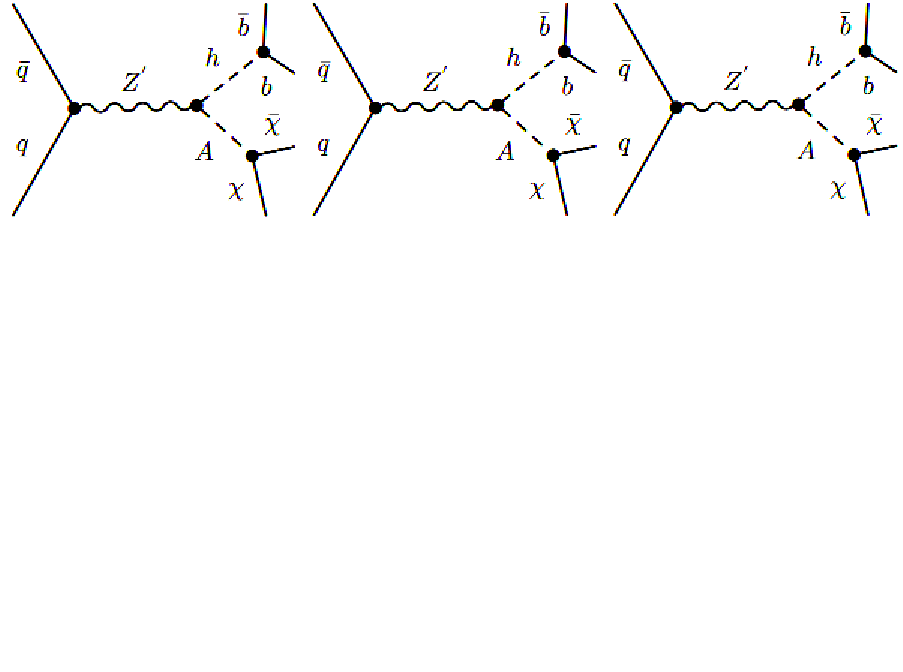
\includegraphics[width=0.9\textwidth]{Figures/2/Fey_monoH.pdf}
\caption{Figure from $\copyright$ \cite{ATLAS-CONF-2018-039}.}
\label{fig:Fey_monoH}
\end{subfigure}
\begin{subfigure}[t]{0.57\textwidth}
	\centering
	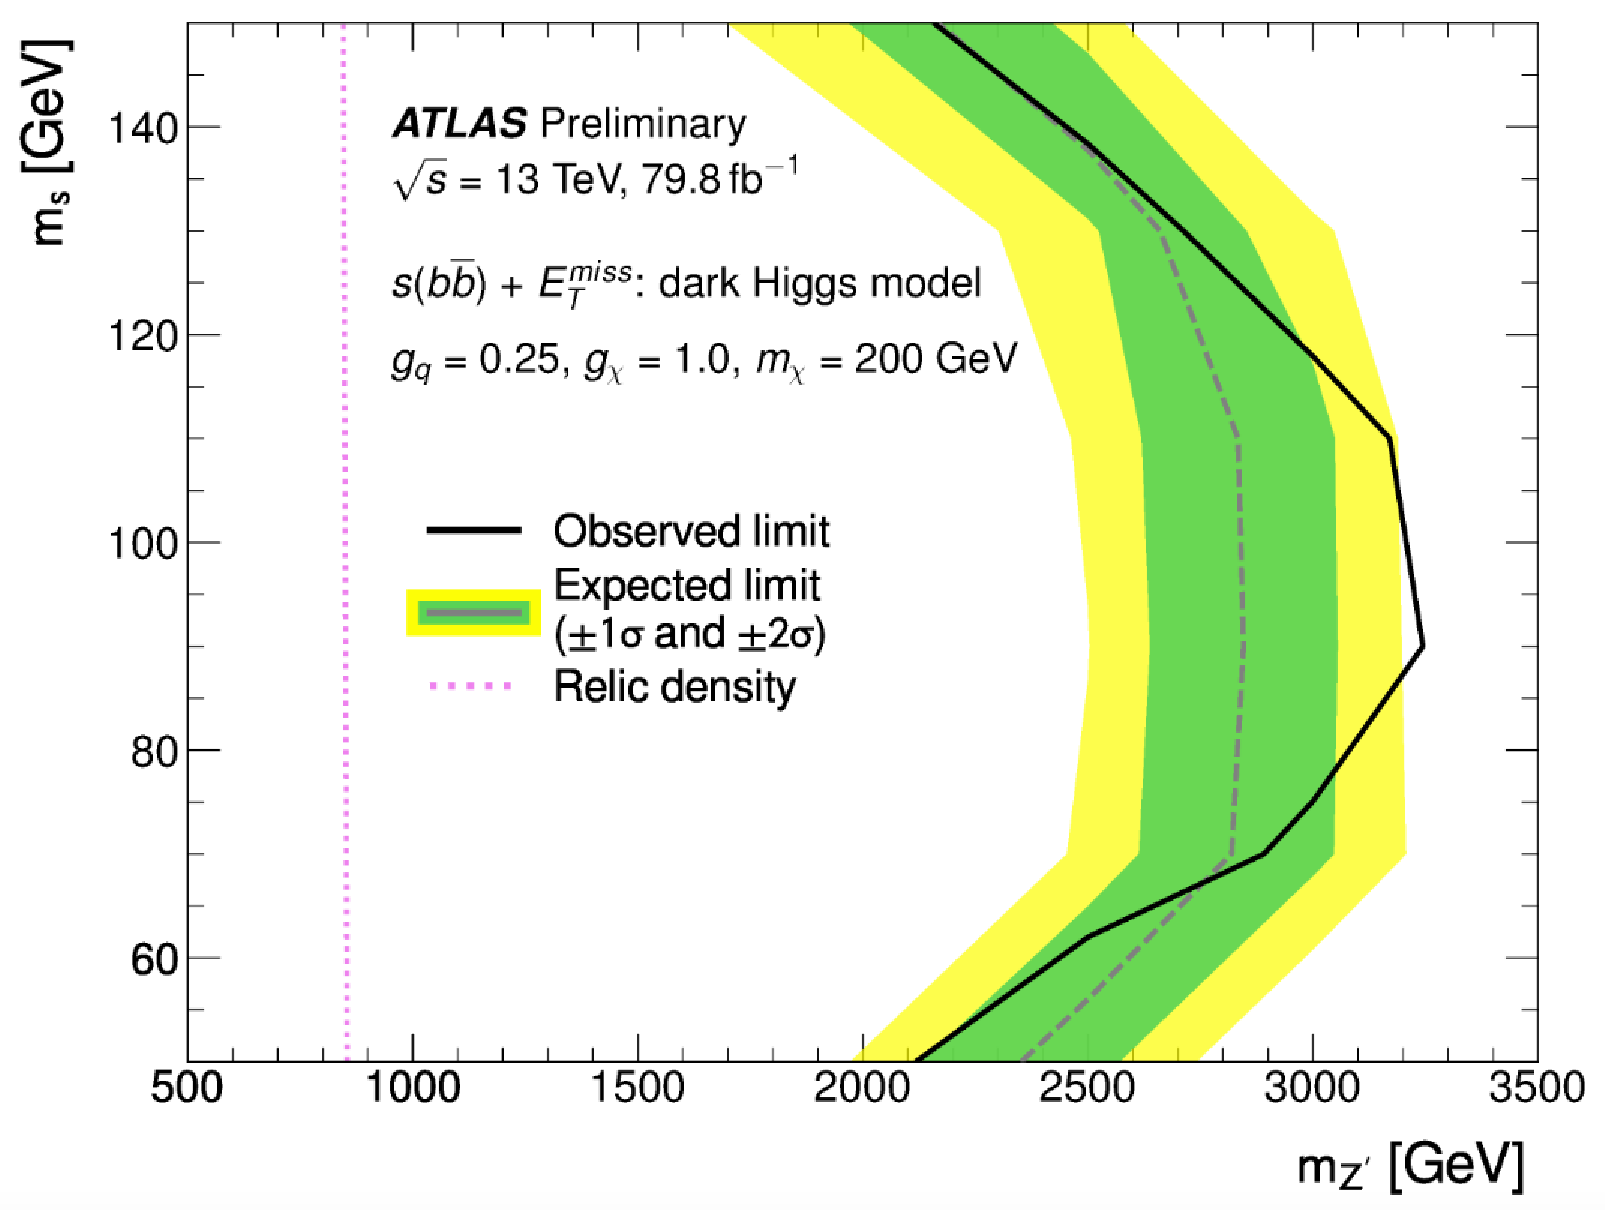
\includegraphics[width=0.99\textwidth]{Figures/2/monosbb_limits.pdf}
\caption{Figure from $\copyright$ \cite{dijet_3}.}
\label{fig:monosbb_limits}
\end{subfigure}
	\caption{Left: Most contributing Feynman diagram for the original DM search \cite{ATLAS-CONF-2018-039} that was re-interpreted in Ref. \cite{ATL-PHYS-PUB-2019-032} to probe the DH model in the \(s\rightarrow bb\) channel. Figure from $\copyright$ \cite{ATLAS-CONF-2018-039}. Right: Exclusion limits on the \ms and \mZp in the DH model in the \(s\rightarrow bb\) channel.  Values of \ms and \mZp to the left of the solid black line are excluded by the search. The dashed pink line reproduces the relic density of DM observed in the Universe for choices of coupling constants \gchi and \(g_q\) in the model. Figure from $\copyright$ \cite{ATL-PHYS-PUB-2019-032}.}
	\label{fig:monosbb_DH_search}
\end{figure}

There is also a dedicated search in the \(s\rightarrow bb\) channel under development within the ATLAS collaboration. In addition to optimizing the search strategy to maximize the sensitivity to the DH model, this search also plans to improve upon the earlier search by scanning over additional model parameters such as \(g_q\) and \mchi that were fixed in the earlier search, with the values of these additional parameters optimized to maximize the sensitivity of the search to the DH model while reproducing the observed relic abundance of DM in the Universe. 

\subsubsection{\(s\rightarrow WW\) and \(s\rightarrow ZZ\) Channels}

The \(s\rightarrow WW\) and \(s\rightarrow ZZ\) (\(s\rightarrow VV\)) channels which collectively dominate the branching fraction for \(s\) decays for \(\ms>160\GeV\) are somewhat more complex in terms of their final state in the detector compared with the \(s\rightarrow bb\) channel because, whereas the dijet \(b\bar{b}\) pair in the latter decay channel will directly hadronize in the calorimeter to produce a characteristic signature of either two distinct hadronic jets or one two-pronged jet\footnote{see Section \ref{sec:had_calo} for more details on hadronic jets in the calorimeter}, the vector bosons in the \(s\rightarrow WW\) and \(s\rightarrow ZZ\) final states can decay via several possible channels, which leads to a number of distinct final states in the detector for these \(s\rightarrow VV\) channels. For this reason, a number of different LHC searches in the \(s\rightarrow VV\) channels have been completed or are ongoing, each of which targets only a subset of the \(VV\) decay modes.  

Table \ref{tab:diboson_decay_modes} summarizes the available decay channels for the \(WW\) and \(ZZ\) final states, as well as the branching fraction of each channel and the details of completed or ongoing efforts to search for the DH model in each \(VV\) decay channel. Figure \ref{ig:mono_sVV_limits} shows the range of \((\ms, \mZp)\) excluded, for \(\mchi=200~\GeV\), by the completed searches by ATLAS in the \(s\rightarrow VV(q\bar{q}q\bar{q})\) channel \cite{monos_had_paper}, and by CMS in the \(s\rightarrow WW(\ell\nu\ell\nu)\) channel \cite{cms_monos_lep}. As would be expected on the basis of the branching fractions in Figure \ref{fig:higgs_branching_fractions}, these searches exclude parameter space roughly in the range \(\ms > 160~\GeV\). The search presented in this thesis, which covers the \(s\rightarrow WW\) decay channel in the semileptonic final state (\(WW\rightarrow q\bar{q}\ell\nu\)), complements these existing searches, and extends the excluded range of \ms and \mZp. 


\begin{table}[hp]
\centering
\caption{Summary of decay channels for \(WW\) and \(ZZ\) pairs and their branching fractions}
\label{tab:diboson_decay_modes}
\small{
\begin{tabular}{l l p{5cm} }
\toprule
\multirow{2}{*}  \textbf{\textbf{Decay channel}} & \textbf{Branching fractions \cite{PDG_2018}} & \textbf{Search effort(s)} \\
 & \textbf{(from WW or ZZ pair)} & \\
\midrule
\multirow{2}{*}  {\( WW \rightarrow q\bar{q} q\bar{q} \)} & 0.45 & ATLAS published search: Ref. \cite{monos_had_paper} \\
\(ZZ\rightarrow q\bar{q}q\bar{q}\) & 0.49 & \\
\midrule
\(WW\rightarrow q\bar{q}\ell\nu\) (\(\ell=e\text{ or }\mu\)) & 0.29 & This thesis \\
\midrule
\(ZZ\rightarrow q\bar{q}\ell\ell\) (\(\ell=e\text{ or }\mu\)) &0.094 & Ongoing within ATLAS collaboration \\
\midrule
\(ZZ\rightarrow q\bar{q}\nu\nu\) &0.14 & N/A (expected sensitivity too low) \\
\midrule
\(WW\rightarrow \ell\nu\ell\nu\) (\(\ell=e\text{ or }\mu\)) & 0.046 & CMS published search: Ref. \cite{cms_monos_lep}. Effort also ongoing within ATLAS collaboration. \\
\midrule
\(ZZ\rightarrow LLLL\) (\(L=\ell\text{ or }\nu\)) & 0.071 & N/A (expected sensitivity too low) \\
\bottomrule
\end{tabular}}
\end{table}

\begin{figure}[hp]
	\centering
\begin{subfigure}[t]{0.53\textwidth}
	\centering
	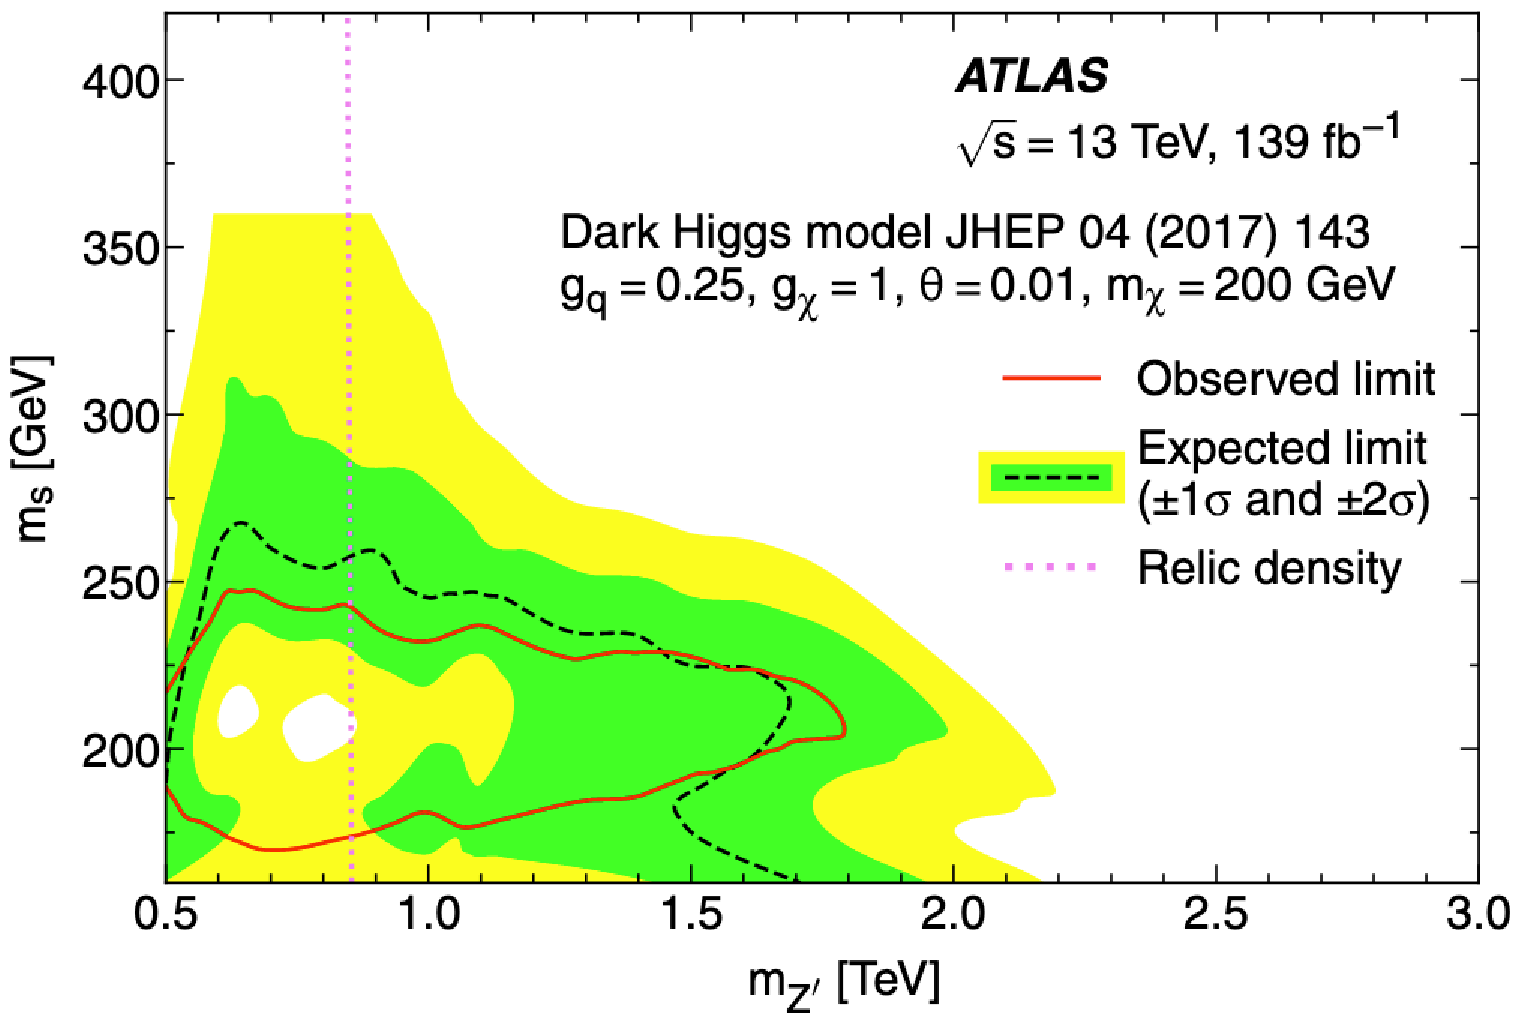
\includegraphics[width=0.9\textwidth]{Figures/2/monos_had_limits.pdf}
\caption{Exclusion limits from search in \(s\rightarrow VV(q\bar{q}q\bar{q})\) channel. Figure from $\copyright$ \cite{monos_had_paper}.}
\label{fig:monosVV_had_limits}
\end{subfigure}
\begin{subfigure}[t]{0.45\textwidth}
	\centering
	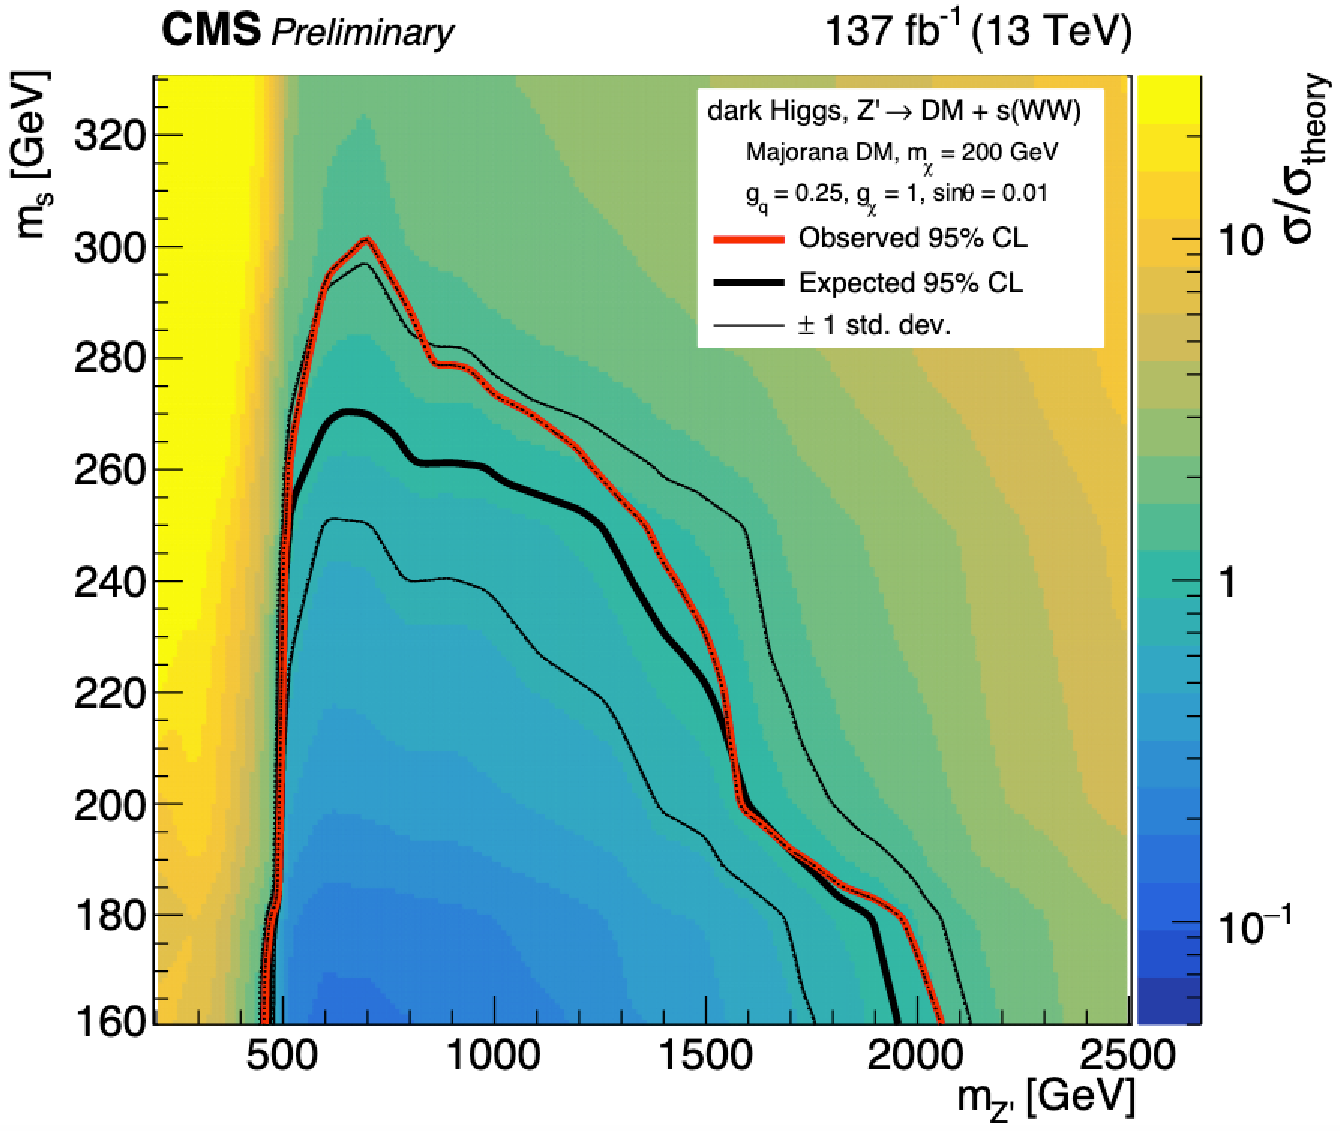
\includegraphics[width=0.99\textwidth]{Figures/2/monos_lep_limits.pdf}
\caption{Exclusion limits from search in \(s\rightarrow WW(\ell\nu\ell\nu)\) channel. Figure from $\copyright$ \cite{cms_monos_lep}.}
\label{fig:monosWW_lep_limits}
\end{subfigure}
	\caption{Range of \((\ms, \mZp)\) in the DH model excluded by searches performed by ATLAS in the \(s\rightarrow VV(q\bar{q}q\bar{q})\) channel (left), and by CMS in the \(s\rightarrow WW(\ell\nu\ell\nu)\) channel (right), for the following choices of remaining parameters in the model: \(g_q=0.25\), \(\gchi=1\), \(\sin\theta=0.01\), \(\mchi=200~\GeV\).}
	\label{fig:mono_sVV_limits}
\end{figure}

